% Created 2016-01-27 Wed 13:49
\documentclass[11pt]{article}
\usepackage[utf8]{inputenc}
\usepackage[T1]{fontenc}
\usepackage{fixltx2e}
\usepackage{graphicx}
\usepackage{grffile}
\usepackage{longtable}
\usepackage{wrapfig}
\usepackage{rotating}
\usepackage[normalem]{ulem}
\usepackage{amsmath}
\usepackage{textcomp}
\usepackage{amssymb}
\usepackage{capt-of}
\usepackage{hyperref}
\usepackage{tikz}
\usepackage{fancyhdr}
\usepackage[left=2cm,right=2cm,top=2cm,bottom=2cm]{geometry}
\renewcommand\vec{\mathbf}
\newcommand\leftidx[3]{{\vphantom{#2}}#1#2#3}
\newenvironment{example}[1]{\vspace{0.2in}\hrule\vspace{0.1in}\noindent\emph{Example:} #1 \\}{\vspace{0.1in}\hrule\vspace{0.2in}}
\pagestyle{fancyplain}
\cfoot{{\it ENGY 5050, Nuclear Reactor Physics, UMass Lowell}}
\author{Justin Pounders}
\date{\today}
\title{ENGY 5050}
\hypersetup{
 pdfauthor={Justin Pounders},
 pdftitle={ENGY 5050},
 pdfkeywords={},
 pdfsubject={},
 pdfcreator={Emacs 24.5.1 (Org mode 8.3.2)}, 
 pdflang={English}}
\begin{document}

\maketitle
\tableofcontents


\section{Neutron-Nucleus Reactions}
\label{sec:orgheadline11}
\subsection{Introduction}
\label{sec:orgheadline1}
A neutron striking a nucleus may elicit a number of different reactions.  The types of reactions may be broadly divided into \emph{absorption} and \emph{scattering} reactions.  Absorption reactions are those in which the neutron is integrated into the nucleus, forming a new nucleus.  Normally this results in an excited, unstable nucleus.  The most common way for the nucleus to alleviate the pressure of the new nucleon is through emission of a photon.  The neutron never re-emerges, so this type of reaction is called a \emph{capture} reaction.  For fissile isotopes, the absorption process normally causes the nucleus to split violently into two pieces, or in other words, \emph{fission}.

Scattering-type reactions can be broadly divided into two categories: \emph{elastic} and \emph{inelastic}.  Elastic scattering may be viewed as a classical collision between two solid, non-deformable objects.  Billiard balls are the prototypical example.  Because neither object is "deformed" or excited, energy and linear momentum are conserved in the system.  This is in contrast to inelastic collisions.  

In inelastic scattering reactions, the neutron is actually temporarily absorbed into the nucleus, bringing the nucleus to a compound, excited state.  The compound nucleus then relaxes by emitting both a neutron \emph{and} a photon within a small fraction of a second.  The absorption-reemission process is so fast (with respect to all other time scales of neutron transport) that it may safely be regarded as instantaneous.  Because of the photon emission, neither the kinetic energy nor the momentum of the neutron-nucleus system is conserved.

Nuclear interactions are typically labeled by identifying the target nucleus, the incoming projectile/particle, particles emitted after the reaction, and the nucleus remaining when the dust settles.  For example, given a nucleus \(A\) that is struck by a particle \(p\) leading to the emission of particle \(q\) and a new nucleus \(B\) one would write \(A(p,q)B\).  If the nuclei \(A\) and \(B\) are implicitly assumed then we may simply identify the reaction as a \((p,q)\) reaction.  Thus our reaction hierarchy so far may be written as

\begin{itemize}
\item Absorptions
\begin{itemize}
\item Capture, \((n,\gamma)\)
\item Fission, \((n,f)\)
\end{itemize}
\item Scattering
\begin{itemize}
\item Elastic scattering, \((n,n)\)
\item Inelastic scattering, \((n,n')\)
\end{itemize}
\end{itemize}

Note that we have abused the original notation somewhat (this is standard) by writing \(f\) in place of an ejected particle to denote fission.  We have also written \(n'\) as the ejected particle in inelastic scattering as a reminder that the ejected particle will in general \emph{not} be the same neutron that struck the nucleus.  In some cases, high-energy inelastic scattering reactions may in fact yield more than one neutrons, in which would be denoted \((n,2n)\), \((n,3n)\), etc. with no apostrophe on the ejected particles.

\subsection{Scattering Reactions}
\label{sec:orgheadline9}
To describe the kinematics of neutron-nucleus scattering we will begin with several assumptions.
\begin{enumerate}
\item Relativistic effects can be neglected.  The kinetic energies of neutrons emitted from fission are low enough so that the space-time effects described by relativity may be neglected.
\item Neutron-neutron interactions will be neglected.  Because the density of nuclei in a reactor is much higher than the density of neutrons, neutrons are much more likely to collide with nuclei than they are with other neutrons.
\item Neutrons travel in straight lines between collisions.  This assumption holds because neutrons are neutrally-charged particles and the effect of gravity on neutron trajectories is negligible.
\item Reactors materials are isotropic.  This means that a material has no preferred orientation.  On the scale of neutron-nucleus interactions in a reactor this is a valid assumption.
\end{enumerate}

\subsubsection{Scattering Kinematics}
\label{sec:orgheadline2}

Let us now consider the specific kinematics associated with scattering.
\begin{description}
\item[{\(\vec{V}_n\), \(\vec{V}_n'\) :}] initial and final velocity of the neutron.
\item[{\(E\), \(E'\) :}] initial and final kinetic energy of the neutron.
\item[{\(\vec{V}_A\), \(\vec{V}_A'\) :}] initial and final velocity of the nucleus.
\end{description}
We also define the angles \(\gamma\), \(\theta\), and \(\psi\) as shown in Figure \ref{fig::scatteringLAB}.

\begin{figure}
\centering
\begin{tikzpicture}[x=0.25in,y=0.25in,scale=0.75]
  \draw (3,0) circle [radius=1];
  \draw (3,0) node {\large n};
  \draw [->,thick] (4.5,0) -- (9.5,0);
  \draw (7.25,1) node {$\vec{V}_n$};

  \draw (15,-5) circle [radius=2];
  \draw (15,-5) node {\huge A};
  \draw [->,thick] (13,-3) -- (10.5,-0.5);
  \draw (11,-2) node {$\vec{V}_A$};

  \draw[dashed] (10,0) -- (18,0);

  \draw (12,0) arc [start angle=0, end angle=-45, radius=2];
  \draw (12.3,-1) node {$\gamma$};

  \draw (15.77,-12.11) circle [radius=1];
  \draw (15.77,-12.11) node {\large n};
  \draw [<-,thick] (14.5,-12.75) -- (10,-15);
  \draw (11.75,-13) node {$\vec{V}_n$};

  \draw (14.87,-18.25) circle [radius=2];
  \draw (14.87,-18.25) node {\huge A};
  \draw [<-,thick] (13,-17) -- (10,-15);
  \draw (11,-16.5) node {$\vec{V}_A$};

  \draw[dashed] (2,-15) -- (18,-15);

  \draw (12,-15) arc [start angle=0, end angle=-33.69, radius=2];
  \draw (12.34,-15.7) node {$\psi$};

  \draw (11.5,-15) arc [start angle=0, end angle=26.57, radius=1.5];
  \draw (12.3,-14.4) node {$\theta$};
\end{tikzpicture}
\caption{Neutron-nucleus collision in LAB coordinates.}
\label{fig::scatteringLAB}
\end{figure}

The analysis of scattering kinematics is greatly simplifed by working in the center-of-mass reference frame (CM) rather than the laboratory reference frame (LAB).  The origin in the CM reference frame is 
\begin{align}
  \vec{r}_{CM} = \frac{1}{A+1} \left( \vec{r}_n + A\vec{r}_A \right)
\end{align}
where \(\vec{r}_n\) and \(\vec{r}_A\) are the positions of the neutron and the nucleus, respectively, and \(A\) is the atomic mass ratio of the nucleus (i.e., the ratio of the mass of the nucleus to the mass of the neutron).  Consequently we may deduce that the origin of the CM system is moving with a velocity of
\begin{align}
  \vec{V}_{CM} = \frac{1}{A+1} \left(\vec{V}_n + A\vec{V}_A \right).
\end{align}

The velocities of the neutron and nuclear in the CM system are given by the following relations:
\begin{subequations}
\begin{align}
  \vec{v}_n  &= \vec{V}_n - \vec{V}_{CM} \\
  \vec{v}_n' &= \vec{V}_n' - \vec{V}_{CM} \\ 
  \vec{v}_A  &= \vec{V}_A - \vec{V}_{CM} \\
  \vec{v}_A' &= \vec{V}_A' - \vec{V}_{CM}
\end{align}
\label{eq:cmDefs}
\end{subequations}
We will also define the \emph{relative} velocity between the neutron and nucleus, which is the same in both the CM and LAB systems:
\begin{align}
  \vec{V}_R = \vec{V}_n - \vec{V}_A
\end{align}
This definition allows us to write the CM neutron and nucleus velocities as
\begin{subequations}
\begin{align}
  \vec{v}_n = \frac{A}{A+1}\vec{V}_R \\
  \vec{v}_A = \frac{-1}{A+1}\vec{V}_R
\end{align}
\label{eq:cmVelRel}
\end{subequations}
Thus in the CM system, both neutron and nucleus are moving along the same line in opposite directions before the collision, as shown in Figure \ref{fig::scatteringCM}.

\begin{figure}
\centering
\begin{tikzpicture}[x=0.25in,y=0.25in,scale=0.75]
  \draw (3,0) circle [radius=1];
  \draw (3,0) node {\large n};
  \draw [->,thick] (4.5,0) -- (9.5,0);
  \draw (7.25,1) node {$\vec{v}_n$};

  \draw (15.5,0) circle [radius=2];
  \draw (15.5,0) node {\huge A};
  \draw [->,thick] (13,0) -- (10.5,0);
  \draw (12,1) node {$\vec{v}_A$};


  \draw (15.77,-10.11) circle [radius=1];
  \draw (15.77,-10.11) node {\large n};
  \draw [<-,thick] (14.5,-10.75) -- (10,-13);
  \draw (11.75,-11) node {$\vec{v}_n'$};

  \draw (5.3,-15.35) circle [radius=2];
  \draw (5.3,-15.35) node {\huge A};
  \draw [<-,thick] (7.3,-14.34) -- (10,-13);
  \draw (9.8,-14.2) node {$\vec{v}_A'$};

  \draw[dashed] (2,-13) -- (18,-13);

  \draw (11.5,-13) arc [start angle=0, end angle=26.57, radius=1.5];
  \draw (12.3,-12.4) node {$\varphi$};
\end{tikzpicture}
\caption{Neutron-nucleus collision in CM coordinates.}
\label{fig::scatteringCM}
\end{figure}

Consider now the kinetic energy of the system before the collision.  Letting the variable, \(e\), denote the kinetic energy of a particle in the CM system (i.e., relative to the CM velocity) we  have
\begin{align}
  e_n + e_A = e_{\text{exc}}
\end{align}
where the subscripts are used in the same way as they were in the velocity variables.  The new variable \(e_{\text{exc}}\) is called the \emph{excitation energy}, which is the energy that is available for the reaction, and may be written
\begin{align}
  e_{\text{exc}} = \frac{1}{2} \frac{mA}{A+1}V_R^2
\end{align}
where \(m\) is the mass of a neutron.

\subsubsection{Elastic Scattering}
\label{sec:orgheadline4}
We will now assume that linear momentum is conserved through the collision.  In the LAB system this means
\begin{align}
  \vec{V}_n + A\vec{V}_A = \vec{V}_n' + A\vec{V}_A'
\end{align}
By using the definitions in Eq. \eqref{eq:cmDefs} we see that this relationship carries over to CM system, allowing us to write
\begin{align}
  \vec{v}_n + A\vec{v}_A = \vec{v}_n' + A\vec{v}_A'
\end{align}
Writing the left-hand-side of this expression (i.e., the pre-collision linear momentum) in terms of the relative velocity reveals that net linear momentum both before and after the collision is zero:
\begin{align}
  \frac{A}{A+1}\vec{V}_R - \frac{A}{A+1}\vec{V}_R = \vec{0}
\end{align}
This means that
\begin{align}
  \vec{v}_n = -A \vec{v}_A, \\
  \vec{V}_n' = -A \vec{v}_A'.
\end{align}

Let us now additionally assume conservation of kinetic energy before and after the collision.  That is, 
\begin{align}
  e_n + e_A = e_n' + e_A' = e_{\text{exc}}.
\end{align}
Using Eq. \eqref{eq:cmVelRel}, we find that 
\begin{align}
  v_n = v_n' = \frac{A}{A+1}V_R,
\end{align}
and
\begin{align}
  v_A = v_A' = \frac{1}{A+1}V_R.
\end{align}

\paragraph{Stationary Target Nucleus}
\label{sec:orgheadline3}
Consider the special case where target nucleus is stationary, i.e. \(\vec{V}_A = 0\).  From the previous section we know that
\begin{align}
  \vec{V}_{CM} = \frac{1}{A+1} \vec{V}_n, \text{ and} \\
  v_n = v_n' = \frac{A}{A+1}V_n.
\end{align}
We can sketch a diagram of the relationship between the LAB and CM velocities and the velocity of the center-of-mass.

\begin{figure}
\centering
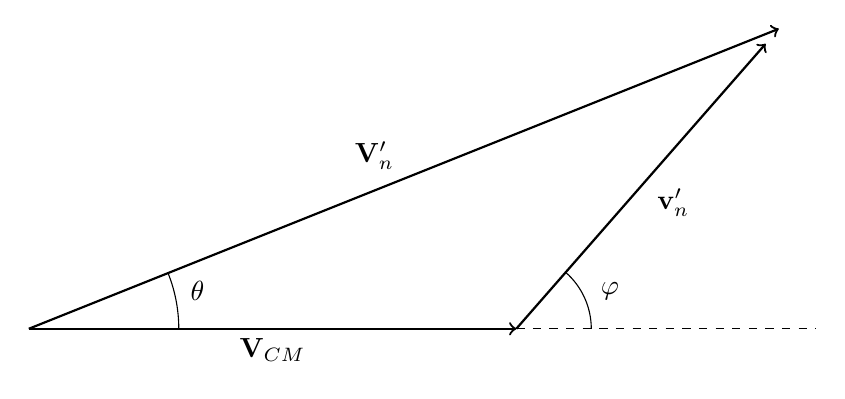
\begin{tikzpicture}[x=0.25in,y=0.25in,scale=0.75]
  \draw [->,thick] (0,0) -- (13,0);
  \draw (6.5,0) node[anchor=north] {$\vec{V}_{CM}$};

  \draw [->,thick] (0,0) -- (20,8);
  \draw (10,4) node[anchor=south east] {$\vec{V}_n'$};

  \draw [->,thick] (13,0) -- (19.65,7.6);
  \draw (16.5,4) node[anchor=north west] {$\vec{v}_n'$};

  \draw [dashed] (13,0) -- (21,0);

  \draw (15,0) arc [start angle=0, end angle=48.84, radius=2];
  \draw (15.5,1) node {$\varphi$};

  \draw (4,0) arc [start angle=0, end angle=21.8, radius=4];
  \draw (4.5,1) node {$\theta$};
\end{tikzpicture}
\caption{Relationship between final neutron velocities in LAB and CM.}
\label{fig::scatteringVelLABvsCM}
\end{figure}

From this diagram, we can apply the law of cosines to find
\begin{equation}
  V_n'^2 = V_{CM}^2 + v_n'^2 + 2 V_{CM}v_n'\cos(\pi-\varphi)
\end{equation}
which simplifies to
\begin{equation}
  V_n'^2 = \left[ \frac{A^2+1}{(A+1)^2} + 2 \frac{A}{(A+1)^2}\cos(\varphi) \right] \vec{V}_n^2.
\end{equation}
An immediate implication of this expression is the relationship between the final and initial kinetic energies of the neutron and the scattering angle in the CM system:
\begin{align}
  \frac{E_n'}{E_n} = \frac{V_n'^2}{\vec{V}_n^2}
                   = \frac{(1+\alpha) + (1-\alpha) \cos(\varphi)}{2}
\end{align}
where
\begin{align}
  \alpha = \left( \frac{A-1}{A+1} \right)^2
\end{align}

To understand this a bit better let's consider a few limiting cases.
\begin{description}
\item[{\(A=1\) :}] This is the case of a neutron scattering off a hydrogen nucleus, and \(\alpha = 0\).  For a glancing collision, the angle of deflect (\(\varphi\) or \(\theta\)) will be very small.  Thus \(E_n' \approx E_n\) and no appreciable energy is lost in the collision.  For a direct hit, in which case the neutron bounces straight back (\(\varphi = \theta = \pi\)) we have \$E\(_{\text{n}}\)' = 0\$--the neutron lost \emph{all} of its energy in a single collision.
\item[{\(A>>1\) :}] In this case the neutron hits something big, and \(\alpha \approx 1\).  Under these circumstances \(E_n' \approx E_n\) \emph{regardless} of the deflection angle.  Think of throwing a tennis ball against a brick wall.
\end{description}

Another important ramification is that for any fixed size of the target nucleus, \(A\), their is a limited range of possible final energies for the neutron.  The largest energy loss will occur when the neutron is scattered directly backward, in which case \(E_n' = \alpha E_n\).  On the other hand, for a small-angle glancing collision, the final energy will be only slightly less than the initial energy and \(E_n' \approx E_n\).  Note that under our current assumptions (namely, that the target nucleus is stationary) the neutron will never \emph{gain} energy.

The preceding work shows us that the amount of energy lost by a neutron depends on the mass of the target nucleus and the cosine of the deflection angle in the CM system.  We can derive a similar relationship between the energy loss and the cosine of the deflection angle in the LAB system, which is often more useful from simulation perspective.

Again starting with the diagram and using the law of cosines we have
\begin{align}
  v_n'^2 = V_n'^2 + V_{CM}^2 - 2 V_n' V_{CM} \cos\theta.
\end{align}
This simplifies to 
\begin{align}
  \left( \frac{A}{A+1} \right)^2 V_n^2 = V_n'^2 + \left( \frac{1}{A+1} \right)^2 V_n^2 - \frac{2}{A+1} V_n' V_n \cos\theta.
\end{align}
Multiplying by the mass of a neutron squared divided by four (to get an expression in terms of energies) and solving for \(\cos\theta\) yields
\begin{align}
  \cos\theta = \frac{1}{2}\left( A+1 \right) \sqrt{\frac{E_n'}{E_n}}
             - \frac{1}{2}\left( A-1 \right) \sqrt{\frac{E_n}{E_n'}}.
\end{align}

\subsubsection{Reactions Involving a Compound Nucleus}
\label{sec:orgheadline5}
Elastic scattering may be viewed a billiard ball collision.  The neutron and nucleus exchange kinetic energy and linear momentum but nothing else.  In collisions such as inelastic scattering, neutron capture, and fission however, the neutron and nucleus combine to form a new, compound nucleus.  Moreover, this compound nucleus will generally be in an \emph{excited} state, having received additional internal energy from the collision.  We may write such a reaction as
\begin{align}
  \leftidx{^A_Z}{X}{} + \leftidx{^1_0}{n}{} 
  \rightarrow \leftidx{^{A+1}_Z}{X}{^*}
\end{align}
where the * symbol is used to indicate an excited state.  The first reaction in this process is the absorption of a neutron into the target nucleus.  The resultant excited nucleus will then decay, generally on a time scale of \(10^{-14}\) to \(10^{-21}\) seconds.

There are two sources of the excitation energy in a compound nucleus.  First, there is the kinetic energy that is available to the reaction.  This energy, \(e_{\text{exc}}\), is the total pre-collision kinetic energy of the neutron and nucleus in the CM reference frame.  Second, there is a potential source of energy arising from the change in binding energy between the original and compound nuclei.  This change in energy may be expressed as
\begin{align}
  \Delta BE = \left[ M(A,z) + m_n - M(A+1,Z) \right] c^2
\end{align}
where \(M(A,Z)\) is the mass of nucleus \(\leftidx{^A_Z}{X}{}\), \(m_n\) is the mass of the neutron and \(c\) is the speed of light in a vacuum.  Thus the total energy available to the reaction is \(e_{\text{exc}} + \Delta BE\).

Figure \ref{fig::compoundNucleus} shows a cartoon depicting the excitation of a nucleus following neutron capture and three possible de-excitation processes (also called \emph{decay channels}).  Elastic scattering has already been discussed, and as we will see, can be treated as a special case of inelastic scattering, which we will now discuss.
\usetikzlibrary{decorations.pathmorphing}
\begin{figure}
\centering
\begin{tikzpicture}[x=0.25in,y=0.25in,scale=0.75]
  \draw (17,0) node [anchor=north] {$\leftidx{^{A+1}_Z}{X}{}$};
  \draw (14,0) -- (20,0);
  \draw (14,6) -- (20,6);
  \draw (14,11) -- (20,11);
  \draw (14,15) -- (20,15);
  \draw (14,18) -- (20,18);
  \draw (14,20) -- (20,20);
  \draw (14,22) -- (20,22);
  \draw (14,23.5) -- (20,23.5);
  \draw (14,0) -- (14,25);
  \draw (20,0) -- (20,25);

  \draw (7,17) node [anchor=north] {$\leftidx{^A_Z}{X}{}$};
  \draw (4,17) -- (10,17);
  \draw (4,21) -- (10,21);
  \draw (4,24) -- (10,24);
  \draw (4,17) -- (4,25);
  \draw (10,17) -- (10,25);

  \draw [dashed] (14,23.5) -- (0,23.5);
  \draw [dashed] (20,17) -- (0,17);
  \draw [dashed] (14,0) -- (0,0);

  \draw [<->,thick] (2,0) -- (2,17);
  \draw (2,8.5) node [fill=white] {$\Delta BE$};

  \draw [<->,thick] (2,17) -- (2,23.5);
  \draw (2,20.25) node [fill=white] {$e_\text{exc}$};

  \draw [->,thick] (15,23.5) -- (6,21);
  \filldraw [fill=white, draw=black] (12,22.6) circle [radius=0.15in];
  \draw (12,22.6) node {1};

  \draw [->,thick] (16,23.5) -- (8,17);
  \filldraw [fill=white, draw=black] (12,20.25) circle [radius=0.15in];
  \draw (12,20.25) node {2};

  \draw [->,decorate,decoration={snake}] (6,21) -- (6,17);
  \draw [->,decorate,decoration={snake}] (17,23.5) -- (17,15);
  \draw [->,decorate,decoration={snake}] (18,23.5) -- (18,11);
  \draw [->,decorate,decoration={snake}] (19,23.5) -- (19,6);
  \filldraw [fill=white, draw=black] (17.8,10) circle [radius=0.15in];
  \draw (17.8,10) node {3};

  \draw [->] (22,0) -- (22,4);
  \draw (22,2) node [anchor=west] {$E$};
\end{tikzpicture}
\caption{Formation of a compound nucleus following neutron capture.  The decay channels shown are \textcircled{1} inelastic scattering, \textcircled{2} elastic scattering, and \textcircled{3} radiative capture.}
\label{fig::compoundNucleus}
\end{figure}

\subsubsection{Inelastic Scattering}
\label{sec:orgheadline6}
Inelastic scattering involves the formation of a compound nucleus which subsequently decays through the emission of a neutron and one or more photons (\(\gamma\) rays):
\begin{align}
  \leftidx{^A_Z}{X}{} + \leftidx{^1_0}{n}{} 
  \rightarrow \leftidx{^{A+1}_Z}{X}{^*}
  \rightarrow \leftidx{^A_Z}{X}{} + \leftidx{^1_0}{n}{} + \gamma
\end{align}
The presence of the photon at the end of this reaction clearly indicates that energy has not been conserved between the neutron-nucleus pair.  What has happened instead, is that upon ejection of the neutron, the \(\leftidx{^A_Z}{X}{}\) was actually left in an excited state and emitted one (or more) photons to return to the ground state.

When considering the energetics of inelastic scattering, note that the final nucleus is simply the original target nucleus.  Thus the role of the change in binding energy has no net effect on the energy of the system.  There was \(e_\text{exc}\) energy available before the collision (from the kinetic energy of the neutron and nucleus) and there is still \(e_\text{exc}\) energy available after the collision, although the photon has appeared and claimed part of the available energy.

A second consideration is that for the compound nucleus to decay into an excited state, there must have been at least enough energy, \(e_\text{exc}\), to bridge the gap between the ground and the first excited state of the original nucleus.  Otherwise there would not have been enough energy available after the neutron emission for the target nucleus to be in an excited state!  This type of reaction is known as a \emph{threshold} reaction, because the energy of the colliding pair must meet a certain "threshold" value before the reaction can take place.  Note that if the compound nucleus emits a neutron and returns the target nucleus to its ground state, then there is no photon emission (which is only a result of de-excitation), thus the total energy of the reaction \(e_\text{exc}\) is shared between the neutron and nucleus as kinetic energy.  This, however, implies overall conservation of kinetic energy between the neutron and nucleus, thus it is an \emph{elastic} scattering event!

\subsubsection{Radiative Capture}
\label{sec:orgheadline7}
A radiative capture reaction is essentially an inelastic neutron scattering \emph{without the neutron}.  That is, the target nucleus absorbs a neutron then de-excites simply by emitting one or more photons:
\begin{align}
  \leftidx{^A_Z}{X}{} + \leftidx{^1_0}{n}{} 
  \rightarrow \leftidx{^{A+1}_Z}{X}{^*} + \gamma
\end{align}
Note that the total amount of energy to be relieved through the emission of photons is \(e_{\text{exc}} + \Delta BE\).

\subsubsection{Fission Reactions}
\label{sec:orgheadline8}
In a fission reaction, the energy \(e_{\text{exc}} + \Delta BE\) is enough to overcome the fission barrier (which is an energy threshold), and the nucleus splits into two fragments plus several free neutrons and photons.  The nuclear configuration of the fission fragments and the number of free neutrons emitted are both statistical quantities.  
\subsection{References}
\label{sec:orgheadline10}
\begin{itemize}
\item \href{Hebert2009}{Hebert}
\item \href{Duderstadt:Hamilton1976}{Duderstadt and Hamilton}
\item \href{Stacey2001}{Stacey}
\end{itemize}

\section{Cross Sections}
\label{sec:orgheadline23}
\subsection{What is a Cross Section?}
\label{sec:orgheadline12}
We have already assumed that neutrons travel along straight trajectories between collisions and argued that this is indeed a valid assumption within studies of nuclear reactor physics.  But how can we characterize the frequency of collisions for neutrons traveling along a given trajectory?  Put another way, if a neutron starts along a trajectory from a known point, how long should we expect it to travel before it experiences a collision.  This is clearly a problem for probability.  Hebert (2009) summarizes the problem nicely.

\begin{quote}
The probablity for a neutron located at \(\vec{r}\) and moving in a material at velocity \(\vec{V}_n\) to undergo a nuclear reaction in a differential element of trajectory \(ds\) is independent of the past history of the neutron and is proportional to \(ds\).
\end{quote}

In concrete terms, let's say that we have a  neutron that starts moving at a fixed velocity a medium  containing a exactly one kind of nucleus.  Then define \(P[ds]\) as the probability that the neutron will experience a collision within a differential distance \(ds\), and consider the following
\begin{itemize}
\item We were told (above) that the probability \(P[ds]\) is proportional to \(ds\).
\item From intuition, we can also convince ourselves that this probability should also be proportional to the number of "target" nuclei present, so let's define \(N\) as the density of nuclei.
\end{itemize}
From these observations we may write
\begin{align}
  P[ds] = \sigma N ds
\end{align}
The quantity \(P[ds]\) is a probability, so it should be unitless.  Given that \(N\) is a density and \(ds\) is length, we can infer that the proportionality constant, \(\sigma\), has units of length squared or area.  The constant \(\sigma\) is called the \emph{microscopic cross section}.  It is common to express the microscopic cross section in units of \emph{barns} (b) where \(1 \text{ b} = 10^{-24} \text{ cm}^2\).

The product of the first two variables appearing on the right-hand-side of the probability definition is called the \emph{macroscopic cross section}, written as
\begin{align}
  \Sigma = \sigma N,
\end{align}
which may be interpreted as the probability \emph{per unit path-length} of a collision.  Thus we may write the probability of a neutron collision over the differential path-length \(ds\) as
\begin{align}
  P[ds] = \Sigma ds.
\end{align}

Next, consider a \emph{population} of neutrons with a density, \(n\).  For now let's assume that all neutrons have the same speed, but they need not be moving in the same direction.  The number of neutrons that will experience a collision within the differential path-length \(ds\) along each of their individual trajectories will be \(P[ds]\) multiplied by the number of neutrons.  If we multiply by the \emph{density} of neutrons rather than the \emph{number} of neutrons then we get the (differential) density of neutron collisions within a (differential) distance \(ds\) of collective neutron travel:
\begin{align}
  dC = \Sigma n ds.
\end{align}
Note the units of (collisions) per unit volume.

Because all neutrons are moving at the same speed, \(V_n\), we may relate the distance \(ds\) (of "collective neutron travel") to a time interval \(dt = \frac{ds}{V_n}\).  Thus the density of neutron collisions is \(dC = \Sigma n V_n dt\).  Dividing by \(dt\) and taking \(dt \rightarrow 0\) gives us an important quantity in reactor physics, called the \emph{reaction rate density}:
\begin{align}
  R = \frac{dC}{dt} = \Sigma n V_n.
\end{align}
Because we have officially taken the limit \(dt \rightarrow 0\) (and correspondingly \(ds \rightarrow 0\)), this quantity is a point-wise, instantaneous value.

The product of neutron density and neutron speed, \(n V_n\), appearing on the right-hand-side of the reaction rate density is a ubiquitous quantity in reactor physics, called the \emph{scalar flux}:
\begin{align}
  \phi = n V_n.
\end{align}

We have previously established that there are several different types of nuclear reactions (radiative capture, elastic and inelastic scattering, etc.)  Each type of reaction is represented by unique microscopic cross section.  For a reaction of type \(x\), for example, we may write the corresponding cross section \(\sigma_x\).  Multiplying by the nuclide density provides the corresponding macroscopic cross section \(\Sigma_x = N \sigma_x\).

If there is more than one type of nuclide present, we may simply add the contributions from each to obtain macroscopic cross section for the mixture:
\begin{align}
  \Sigma_x = \sum_i N_i \sigma_{x,i}.
\end{align}
More over we may sum across all reaction types to obtain the \emph{total} macroscopic cross sections, which is the probability per unit path-length of \emph{any} collision:
\begin{align}
  \Sigma = \sum_x \Sigma_x.
\end{align}

\begin{example}{Derivation of Mean-Free-Path}
Now consider a monoenergetic beam of neutrons with uniform velocity $\vec{V}_n$ impinging normally on the surface of slab with a total macroscopic cross section $\Sigma$.  On average, how far will a neutron travel into the slab before experiencing its first collision?

First construct a balance equation for the uncollided neutron density as a function of $x$.  We know that the rate of neutron removal (with respect to $x$) will be the rate of neutron collisions, and there are no sources of uncollided neutrons inside the slab.  Thus,
\begin{align}
  \frac{dn}{dx} = -\Sigma n(x).
\end{align}
We can solve this equation to determine
\begin{align}
  n(x) = n(0) e^{-\Sigma x}.
\end{align}
The probability that a neutron will reach a distance $x$ without experiencing is a collision is thus
\begin{align}
  p_0(x) = \frac{n(x)}{n(0)} = e^{-\Sigma x}.
\end{align}

Next, the probability of a neutron experiencing its first collision between $x$ and $x+dx$ is the product of (1) the probability of the neutron reaching $x$ and (2) the probability of the neutron colliding between $x$ and $x+dx$:
\begin{align}
  p_c(x)dx = p_0(x) \Sigma dx = \Sigma e^{-\Sigma x} dx.
\end{align}

Finally, the average distance to first collision, which we will call $\lambda$, may be obtained by taking the integral
\begin{align}
  \lambda = \int_0^\infty x p_c(x) dx = \frac{1}{\Sigma}.
\end{align}
The quantity $\lambda$ is called the /mean-free-path/ and, for an infinite, homogeneous medium, is equal to the inverse of the total macroscopic cross section.
\end{example}

\subsection{Resonance}
\label{sec:orgheadline16}
Because of the quantum nature of reality, which is very important at the nuclear scale, a nucleus is not allowed to be excited to an arbitrary energy level.  Rather a nucleus may only sit at certain discrete energy levels, at or above its ground state.  Nuclei in excited states will seek to return to the stable ground state, typically though photon emission, although at high enough energy a neutron or even alpha particle may be emitted.  For some nuclei, the additional energy is sufficient to cause fission.  

Although each excitation level, say \(e_i\), is discrete, it's value is not precisely defined due to the Heisenberg uncertainty principle.  Rather each excited state is associated with an energy width, \(\gamma_i\), that is centered at \(e_i\) and related to the average lifetime of the excited state, \(\tau_i\) by
\begin{align}
  \gamma_i = \frac{\hbar}{\tau_i}.
\end{align}
Note that the average lifetime \(\tau_i\) is equal to the inverse of the decay constant for the excited state.

An excited, compound nucleus at excitation level \(e_i\) with width \(\gamma_i\) may have several options for de-excitation: emitting a photon, a neutron, etc., for example.  Each one of these "options" is called a \emph{decay channel}.  The energy width, \(\gamma_i\), of the excited state may be written as a sum of the widths associated with each possible decay channel:
\begin{equation}
  \gamma_i = \sum_x \gamma_{i,x},
\end{equation}
where \(x\) represents a decay channel.

A discussion of the quantum effects surrounding nucleus formation and de-excitation can quickly become quite involved.  While interesting, that discussion is beyond the objectives of our present endeavor.  Thus the following brief sections will only present a high-level summary of the things it might be good to know as nuclear \emph{engineer}.

Recall that there is \(e^* = e_{\text{exc}} + \Delta BE\) of energy available to a newly-created compound nucleus that has been struck by a neutron.  When \(e^*\) is close to an excitation level \(e_i\) of the compound nucleus--if the available reaction energy puts the compound nucleus rather precisely into an excited state--then we observe a \emph{resonance} condition.  A resonance condition means that is \emph{very likely} that the compound nucleus will be formed at the excited state corresponding to the \(e_i\) level.  Resonance conditions have a significant impact on the likelihood that a reaction will take place, and consequently the cross section for that reaction will be significantly affected.

\subsubsection{Single Level Breit-Wigner Formula}
\label{sec:orgheadline13}
There is a result from quantum mechanics that provides an expression for a reaction cross section in the vicinity of a resonance.  The formula is known as the \emph{single level Breit-Wigner Formula} (SLBW).  The "single level" qualifier belies the assumption the resonance in question is well-separated from nearby resonances.  Conversely, if two energy states are close enough together that their associated energy widths (\(\gamma_i\) \(\gamma_{i+1}\), for example) overlap, then the there will be interference effects between the two states.  This will then lead to more complex expressions for describing the corresponding resonance effects that manifest in the cross sections.

For a reaction of type \(x\) from which there are no emerging neutrons (e.g., radiative capture), the SLBW may be written
\begin{align}
  \sigma_x(e_{\text{exc}}) = \sigma_0 \frac{\gamma_{x,i}\gamma_i}{\gamma_i^2+4(e_\text{ext}-e_i)^2}
\end{align}
where
\begin{align}
 \sigma_0 &= 4\pi \lambda^2 g_J \frac{\gamma_{n,1}(e_\text{exc})}{\gamma_i},  \\
  g_J &= \frac{2J+1}{2(2I+1)}, \text{ and} \\
  \lambda &= \frac{\hbar}{\sqrt{2e_\text{exc} \left( \frac{Am}{A+1} \right)}}.
\end{align}
The quantity \(g_J\) is a statistical factor expressed in terms of the spin of the target nucleus (\(I\)) and compound nucleus (\(J\)).  The parameter \(\lambda\) is the de Broglie wavelength of the incident neutron in the CM system.

For an elastic scattering reaction, the SLBW becomes
\begin{align}
  \sigma_e(e_\text{exc}) = \sigma_p^\ell 
                         + \sigma_0 \left[ \frac{2}{\gamma_i}(e_\text{exc}-e_i) \sin 2\phi_\ell 
                                         + \frac{\gamma_{n,i}}{\gamma_i} -2 \sin^2 \phi_\ell \right] \frac{\gamma_i^2}{\gamma_i^2+4(e_\text{exc}-e_i)^2}
\end{align}
where
\begin{align}
  \sigma_p^\ell = 4\pi \lambda^2 \left( 2\ell + 1 \right) \sin^2 \phi_\ell
\end{align}
is called the \emph{potential} cross section.
In this expressions the quantity \(\ell\) is the integer \emph{angular momentum quantum number}, which enumerates several types of elastic scattering reactions:
\begin{align}
  \ell = 
  \begin{cases}
    0; & s\text{-wave interaction} \\
    1; & p\text{-wave interaction} \\
    2; & d\text{-wave interaction} \\
    \text{etc.} &
  \end{cases}
\end{align}
Most elastic scattering reactions in thermal reactors will be \(s\text{-wave}\) interactions, characterized by relatively low incident neutron energies.  Heavy target nuclei may give rise to higher-waver interactions.  The first few \(\phi_\ell\) \emph{shift factors} are given by
\begin{align}
  \phi_0 &= \frac{a}{\lambda}, \\
  \phi_1 &= \frac{a}{\lambda} - \tan^{-1} \frac{a}{\lambda}, \\
  \phi_2 &= \frac{a}{\lambda} - \tan^{-1} \frac{\frac{3a}{\lambda}}{3 - \left( \frac{a}{\lambda} \right)^2}
\end{align}
where \(a\) is the nucleus \emph{diffusion radius}, which can be thought of as the "radius of influence" of the nucleus.  (A nucleus does not have a well-defined boundary in the quantum world!)

The expressions so far have been defined with respect to the CM system.  Most of us do not live in the center-of-mass world of nuclear collision; we operate in a world that is stationary with respect to \emph{us}, i.e., the LAB system, and would prefer to work accordingly.  The excitation energy \(e_\text{exc}\) in the CM system can be converted to a LAB energy easily:
\begin{align}
  E_\text{exc} = \frac{A+1}{A}e_\text{exc} = \frac{1}{2} m_n V_R^2.
\end{align}
If we assume that the target nucleus is stationary, then \(E_\text{exc}\) is simply the initial kinetic energy of the neutron.

With regard to resonance descriptions, a resonance at \(e_i\) with a width \(\gamma_{x,i}\) for decay channel \(x\) in the CM system becomes the following in the LAB system:
\begin{align}
  E_i &= \frac{A+1}{A} e_i, \\
  \Gamma_{x,i} &= \frac{A+1}{A} \gamma_{x,i}.
\end{align}
The SLBW formulas remain valid in the LAB as long as the lowercase (CM) variables above are replaced by their uppercase (LAB) counterparts.

We will conclude this section by remarking that in the case of a resonance located at an energy \(e_{x,i}\) above the thermal energy range (i.e., >1 eV).  If we assume that that \(a/\lambda << 1\) then only \(s-\text{wave}\) interactions are important.  Then using LAB variables, the SLBW formulas become
\begin{align}
  \label{eq::simpleSLBW1}
  \sigma_x(E_\text{exc}) &=  \sigma_0 \frac{\Gamma_{x,i} \Gamma_i}{\Gamma_i^2 + 4\left(E_\text{exc} - E_i\right)^2} \\
  \label{eq::simpleSLBW2}
  \sigma_e(E_\text{exc}) &= 4\pi a^2 
         + \sigma_0 \frac{2a}{\lambda} \frac{2\Gamma_i\left(E_\text{exc} - E_i\right)}{\Gamma_i^2 + 4\left(E_\text{exc} - E_i\right)^2}
         + \sigma_0 \frac{\Gamma_{n,i} \Gamma_i}{\Gamma_i^2 + 4\left(E_\text{exc} - E_i\right)^2} \;\;.
\end{align}

\subsubsection{Limitations of SLBW}
\label{sec:orgheadline14}
The main assumption of the SLBW was that resonances were well-separated and did not interfere with one another.  In reality this assumption breaks down, especially in heavy target nuclei and high energies (\(\gtrsim 10\) keV).  There is a more accurate representation of closely-spaced resonances called the multilevel Breit-Wigner (MLBW) formula.  The complexity of this formula increases significantly.  The MLBW is, however, often used in computer codes that calculate neutron cross sections for reactor physics applications.

\subsubsection{Resonance Distributions}
\label{sec:orgheadline15}
The location and density of resonances varies by nuclide and energy.  In general both the number and density of resonances increases with larger nuclides and higher incident neutron energies.  Below 1-10 keV resonances are typically separated enough so that experimentalists can determine the location and width of the resonances. At higher energies, however, the resonances become so tightly spaced that is impossible, at present, to distinguish one from the other.  We say that these resonances are \emph{unresolved}, or lie in the \emph{unresolved resonance range}, in contrast to the \emph{resolved resonance range} at lower energies.
\subsection{Non-Stationary Nuclei}
\label{sec:orgheadline20}
In much of our initial discussion on neutron-nuclear interactions we assumed that the target nucleus was stationary (\(\vec{V}_A\)).  Short of being at absolute zero temperature, this is never the case in reality.  If the speed of the neutron is much larger than the speed of the target nucleus this ma be a good assumption, however, so our previous discussions are justified.  At neutron energies below 1 eV the random, thermal motion of the nuclei is not negligible.

\subsubsection{Averaging the Microscopic Cross Section}
\label{sec:orgheadline17}
The velocities of nuclei in thermal equilibrium is described by the Maxwell-Boltzmann probability density function,
\begin{align}
  p(\vec{V}_A) = \left( \frac{mA}{2\pi k T} \right)^\frac{3}{2} \exp\left(-\frac{mAV_A^2}{2kT}\right) 
\end{align}
where
\begin{description}
\item[{\(k\)}] is the Boltzmann constant,
\item[{\(T\)}] is the absolute temperature of the material,
\item[{\(m\)}] is the neutron mass,
\item[{\(A\)}] is the ratio of the nuclear mass to the mass of a neutron.
\item[{\(p(\vec{V}_A)d^3V_A\)}] is the probability for a nucleus to have a velocity within an interval \(d^3V_A\) of \(\vec{V}_A\).
\end{description}

We know that for a fixed neutron speed \(V_n\) the reaction rate for reaction type \(x\) is defined by
\begin{align}
  R_x = N \sigma_x(E_\text{exc}) V_R n,
\end{align}
where \(N\) and \(n\) are the densities of the nuclei and neutrons, respectively.  Note that because we are not assuming a stationary nucleus, we use the relative speed, \(V_R\), which is the speed at which the neutron is approaching the target, \(V_R = V_n - V_A\).  Also recall that the excitation energy  in the LAB is \(E_\text{exc} = \frac{A+1}{A}e_\text{exc} = \frac{1}{2}mV_R^2\) (where \(m\) is the neutron mass), so we may use \(E_\text{exc}\) and \(V_R\) interchangeably as the independent variable in the microscopic cross section.  Thus for a fixed neutron speed \(V_n\) the reaction rate depends on the speed of the target nucleus which is random.  To account for this thermal motion of the nuclei, we can calculate an average reaction rate over the probability distribution of target nuclei:
\begin{align}
  \left<R_x\right> = \int_0^\infty p(\vec{V}_A) N \sigma_x(\left| \vec{V}_n - \vec{V}_A \right|) \left| \vec{V}_n - \vec{V}_A \right| n d^3V_A \;\;,
\end{align}
where the integral is taken over each of the velocity components.  From this average reaction rate we can define a new \emph{effective} microscopic cross section averaged over the motion of the nuclei, which for neutron with speed \(V_n\) is:
\begin{align}
  \bar{\sigma}_x(V_n) = 
  \left<\sigma_x(\left| \vec{V}_n - \vec{V}_A \right|)\right> = 
  \frac{1}{V_n} \int_0^\infty p(\vec{V}_A) \sigma_x(\left| \vec{V}_n - \vec{V}_A \right|) \left| \vec{V}_n - \vec{V}_A \right| d^3V_A \;\;.
\end{align}

Plugging in the Maxwell-Boltzmann distribution into this expression yields
\begin{align}
  \bar{\sigma}_x(V_n) = 
  \frac{1}{V_n} \left( \frac{mA}{2\pi k T} \right)^\frac{3}{2}
  \int_0^{2\pi} \delta \int_0^\infty dV_{xy} V_{xy} \int_{-\infty}^\infty dV_z \exp\left(-\frac{mAV_A^2}{2kT} \right) \sigma_x(V_R) V_R \;\;.
\end{align}
The expression can be simplified somewhat without approximation.  To begin, consider the velocity of the target nucleus decomposed into a radial (\(xy\)) and axial (\(z\)) component:
\begin{align}
  \vec{V}_A = V_{xy} \cos\eta \vec{i} + V_{xy} \sin\eta \vec{j} + V_z \vec{k}
\end{align}
where \(\eta \in \left[0, w\pi\right]\), and
\begin{align}
  d^3V_A = V_{xy} d\eta dV_{xy} dV_z \;\;.
\end{align}
The primary quantity that needs to be evaluated for the averaging is the relative speed.  If we define the coordinate reference frame so that the \(\vec{k}\) unit vector is pointing in the direction of neutron travel then we have
\begin{align}
  V_R = | \vec{V}_n - \vec{V}_A | = \sqrt{V_{xy}^2  + \left(V_n - V_z\right)^2} \;\;.
\end{align}
Additionally,
\begin{align}
  V_A^2 = V_{xy}^2 + V_z^2 = V_R^2 - V_n^2 + 2V_nV_z \;\;.
\end{align}
Finally, changing the variable of integration of the first integral from \(V_{xy}\) to \(E_\text{exc}\) using the relationship
\begin{align}
  E_\text{exc} = \frac{1}{2}m\left[V_{xy}^2 + (V_n - V_z)^2\right]
\end{align}
(which requires changing the bounds of the \(V_z\) integration) and integrating over \(V_z\) yields
\begin{align}\label{eq::avgMicro}
  \bar{\sigma}_x(E) = \frac{1}{\Delta\sqrt{\pi}} \int_0^\infty dE_\text{exc} \sqrt{\frac{E_\text{exc}}{E}} \sigma_x(E_\text{exc}) 
  \left\{ \exp\left[ -\frac{A}{kT}\left(\sqrt{E_\text{exc}} - \sqrt{E} \right)^2 \right] 
         \exp\left[ -\frac{A}{kT}\left(\sqrt{E_\text{exc}} + \sqrt{E} \right)^2 \right]  \right\}
\end{align}
where
\begin{align}
  \Delta = 2 \sqrt{\frac{EkT}{A}} \quad \text{and} \quad E = \frac{1}{2}mV_n^2 \;\;.
\end{align}

\subsubsection{Averaging Resonance Cross Sections}
\label{sec:orgheadline18}
Accounting for the thermal motion of nuclei in resonance cross sections is at the heart of the \emph{Doppler broadening effect}, which is an important player in both steady-state and transient reactor analysis.  In the case of an isolated, narrow resonance above the thermal neutron energy range we can take several further steps to simplify Eq. \eqref{eq::avgMicro}.
\begin{enumerate}
\item If the neutron has a kinetic energy significantly above the average kinetic energy of the nuclei then \(E_\text{exc} \approx E\) and we may assume that \(\exp\left[-\frac{A}{kT}\left(\sqrt{E_\text{exc}} + \sqrt{E}\right)^2\right] << \exp\left[-\frac{A}{kT}\left(\sqrt{E_\text{exc}} - \sqrt{E}\right)^2\right]\).  Consequently we will take
\begin{align}
  \exp\left[-\frac{A}{kT}\left(\sqrt{E_\text{exc}} + \sqrt{E}\right)^2\right] \approx 0 \;\;.
\end{align}
\item Because we have assumed that the resonance is narrow we may assume that the peak energy, \(E_i\), is much greater than the resonance width, \(\Gamma_i\).
\item When \(E_\text{exc}\) is much different than \(E\), the first exponential term in Eq. \eqref{eq::avgMicro} will rapidly tend to a small number.  Thus we may generate a Taylor expansion of \(\left(\sqrt{E_\text{exc}} - \sqrt{E}\right)\) in \(E\) with \(E_\text{exc} = E + \varepsilon\) and \(\varepsilon << E\).
\item We assume \(s-\text{wave}\) interactions and use lab variables so that Eqs. \eqref{eq::simpleSLBW1} and \eqref{eq::simpleSLBW2} may be used.
\item Assume that \(\Gamma_{x,i}\) and \(\Gamma_i\) are constant.  (In reality there is some variation with energy.)
\end{enumerate}
Applying all of these assumptions and approximations leads to
\begin{align}
  \label{eq::dopplerSLBWx}
  \bar{\sigma}_x(E) &= \frac{1}{\Delta \sqrt{\pi}} \sigma_0(E) \frac{\Gamma_{x,i}}{2}
                      \int_{-2E_i/\Gamma_i}^\infty dv \frac{1}{1+v^2} \times \\
                    &\phantom{=}  \exp\left\{ -\frac{A}{kT} \frac{\Gamma_i^2(v-u)^2}{16E}
                                  \left[ 1 - \frac{1}{2}\left( \frac{\Gamma_i(v-u)}{2E} \right)
                                           + \frac{5}{16}\left( \frac{\Gamma_i(v-u)}{2E} \right)^2 + \hdots \right] \right\}
\end{align}
where
\begin{align}
  u = \frac{2}{\Gamma_i}\left(E - E_i\right)
  \quad \text{and} \quad
  v = \frac{2}{\Gamma_i}\left(E_\text{exc} - E_i\right) \;\;.
\end{align}
The lower integration limit can be replaced by \(-\infty\) because \(\Gamma_i << E_i\), leading to the following result:
\begin{align}
  \bar{\sigma}_x(E) = \sigma_0(E) \frac{\Gamma_{x,i}}{\Gamma_i} \psi(u,\alpha,\beta)
\end{align}
where
\begin{align}
  \psi(u,\alpha,\beta) = \frac{1}{\beta\sqrt{\pi}}
                         \int_{-\infty}^\infty dv \frac{1}{1+v^2} \exp\left\{ -\frac{(v-u)^2}{\beta^2}
                         \left[ 1 - \frac{1}{2}\alpha(v-u) + \frac{5}{16}\alpha^2(v-u)^2 + \hdots \right] \right\}
\end{align}
and
\begin{align}
  \alpha = \frac{\Gamma_i}{2E}
  \quad \text{and} \quad
  \beta = \frac{2\Delta}{\Gamma_i} \;\;.
\end{align}
This expression \(\psi(u,\alpha,\beta)\) is called the \emph{generalized Doppler psi function}.

Using the same mathematical treatment, a similar expression can be derivied for the SLBW elastic scattering resonance formula.  The result is
\begin{align}
  \label{eq::dopplerSLBWe}
  \bar{\sigma}_e(E) = 4\pi a^2 + \sigma_0(E)\frac{2a}{\lambda}\phi(u,\alpha,\beta) + \sigma_0(E)\frac{\Gamma_{n,i}}{\Gamma_i}\psi(u,\alpha,\beta)
\end{align}
where
\begin{align}
  \phi(u,\alpha,\beta) = \frac{1}{\beta\sqrt{\pi}}
                         \int_{-\infty}^\infty dv \frac{v}{1+v^2} \exp\left\{ -\frac{(v-u)^2}{\beta^2}
                         \left[ 1 - \frac{1}{2}\alpha(v-u) + \frac{5}{16}\alpha^2(v-u)^2 + \hdots \right] \right\}
\end{align}

Let's take a moment to summarize what has been done in the preceding. We began with the microscopic cross section \(\sigma_x\) that is proportional to the probability of a neutron-nucleus interaction and depends on (equivalent) the excitation energy \(E_\text{exc}\) or the relative speed of the neutron-nucleus pair \(V_R\).  Either parameter is complicated by the fact that the nuclei are moving in essentially a random fashion, describable by the probability function \(p(\vec{V}_A)\).  At thermal equilibrium, this probability function is the Maxwell-Boltzmann distribution, so we can derive an expression for the microscopic cross section that is averaged over the thermal motion of the nuclei.  This was the main result.

Remember that the Maxwell-Boltzmann distribution is a function of the temperature of the material.  Thus as the temperature changes so will the averaged microscopic cross sections.  This phenomenon is called the \emph{Doppler broadening effect}.

The \(\phi-\psi\) Doppler functions derived in this section relied on several important assumptions that will not always hold up in reality.  When situations arise in which these functions are not appropriate one may resort to approximate numerical evaluations of Eq. \ref{eq::avgMicro} directly.  This is commonly done in practice.
\subsubsection{Other Considerations}
\label{sec:orgheadline19}
Many absorption-type cross sections (without resonances in the thermal energy range) vary as \(1/\sqrt{E}\) at low energies.  This is commonly referred to as a ``\(1/v\) energy-dependence,'' where \(v\) refers to the neutron speed.  Surprisingly, the thermal motion of nuclei does \emph{not} affect a cross sections with a \(1/v\) energy variation.  In other words, \(V_n \bar{\sigma_x}(V_n) = V_R\sigma_x(V_R)\) when \(\sigma_x(V_R) \propto V_R^{-1}\).

In stating that the thermal motion of the nuclei follow the Maxwell-Boltzmann distribution, we have implicitly assumed that all nuclei are free to move independently, effectively as molecules in a gas.  Most nuclei, however, are chemically bonded to other nuclei to form molecules.  Molecular motion, including vibration and rotation, for example, affects nuclear motion, so the preceding treatment is not strictly valid.  The primary regime where this becomes important is in neutron scattering at low energy. There are treatments to deal with molecular motion that we will not discuss.  

Arguably the most important example in reactor physics of where molecular motion effects are important is in the thermal scattering of neutrons in water.  An analysts should be aware that water cross sections, and hydrogen bound in water in particular, require special evaluations with respect to temperature.  When obtaining nuclear data for reactor physics calculation, this ``special evaluation'' normally appears as something called a \emph{thermal kernel} or \(S(\alpha,\beta)\) \emph{data} that is tabulated alongside all the other nuclear cross sections.
\subsection{Differential Scattering Cross Sections}
\label{sec:orgheadline21}
Up to this point we have considered scattering cross sections only in the sense as they relate to the probability of a scattering event taking place.  In reactor physics analysis, where we want to track the movement of neutrons through a reactor, we often need more information than this.  In particular, if a neutron scatters we want the ability to predict (in a probabilistic sense) how the scattering event will affect the neutrons energy and direction.

In general we can describe probabilistic scattering kinematics as the product of two functions.  The first is the microscopic cross section for the scattering reaction, which relates the likelihood that the scattering event occur.  We can multiply the cross section by a probability function describing the probability that, upon scattering at a certain energy \(E\), the neutron will emerge from the collision with a new energy \(E'\) and a direction modified by some angle \(\theta\).  We write this as
\begin{align}
  \sigma_n(E \rightarrow E', \mu) = \sigma_n(E)P(E \rightarrow E', \mu)
\end{align}
where \(\sigma_n(E)\) is the microscopic cross section for scattering (elastic or inelastic) and \(P(E \rightarrow E', \mu)dE'd\mu\) is the probability that the neutron will scatter to energy \(E'\) (within an interval \(dE'\) through a deviation cosine \(\mu = \cos\theta\) (within an interval \(d\mu\)).  The quantity \(\sigma_n(E \rightarrow E', \mu)\) is called the \emph{double differential scattering cross section} and is sometimes written as
\begin{align}
  \sigma_n(E \rightarrow E', \mu) \equiv \frac{d^2\sigma_n(E)}{dE'd\mu} \;\;.
\end{align}

\begin{example}{Double-Differential Elastic Scattering Cross Section, Stationary Target}
We previously saw that elastic, isotropic (in CM) scattering off a stationary target leads to the following relationship between energies $E$, $E'$, and CM scattering angle $\varphi$:
\begin{align}
  \frac{E_n'}{E_n} = \frac{V_n'^2}{\vec{V}_n^2}
                   = \frac{(1+\alpha) + (1-\alpha) \cos(\varphi)}{2}
\end{align}
where $\alpha = (A-1)^2/(A+1)^2$.  From this we see that energy and direction change are directly correlated.  The probability density function for a neutron scattering isotropically through the cone created by angle $\varphi$ is given by
\begin{align}
  P(\phi) = \frac{1}{2} \sin\varphi, \quad \phi\in[0,\pi] \;\;.
\end{align}
We see that an increase in $\varphi$ by an amount $d\varphi$ causes a decrease in the exiting energy by an mount $dE'$, and in particular,
\begin{align}
  dE' = - \frac{E(1-\alpha)\sin\varphi}{2}d\varphi \;\;.
\end{align}
Because energy change is directly related to the deviation angle we may write the following expression for the probability that a neutron will be scattered from energy $E$ to energy $E'$:
\begin{align}
  P(E \rightarrow E') dE' = - P(\varphi) d\varphi \;\;.
\end{align}
Substituting in the eliminating $d\varphi$ in favor of $dE'$, then cancelling the differential, and subsituting the expression for $P(\varphi)$ leads to
\begin{align}
  P(E \rightarrow E') = \frac{1}{E(1-\alpha)} \;\;.
\end{align}

What we really want is the probability as a function of energy /and/ angle in the LAB, but we just saw that these are correlated.  We previously derived the following results for the LAB deviation cosine in this scenario:
\begin{align}
  \mu = \cos\theta = \frac{1}{2}\left( A+1 \right) \sqrt{\frac{E_n'}{E_n}}
                   - \frac{1}{2}\left( A-1 \right) \sqrt{\frac{E_n}{E_n'}} \;\;.
\end{align}
Because energy and angle correlated, the function $P(E \rightarrow E', \mu)$ is really a one-parameter function, not two.  Thus we may write
\begin{align}
  P(E \rightarrow E', \mu) = 
  \begin{cases}
    \frac{1}{E(1-\alpha)}\delta\left( \mu - \frac{1}{2}\left( A+1 \right) \sqrt{\frac{E_n'}{E_n}}
                                     - \frac{1}{2}\left( A-1 \right) \sqrt{\frac{E_n}{E_n'}} \right), & \text{if } \alpha E \leq E' \leq E, \\
    0, & \text{otherwise.}
  \end{cases}
\end{align}
The function $\delta(x)$ is the /Dirac delta function/ (see the Appendix for details).
\end{example}

Both \(\sigma_n(E)\) and \(P(E \rightarrow E', \mu)\) depend on the thermal motion of nuclei and there are methods for averaging these quantities over that motion similar to what was shown in the previous section, but these procedures will not be discussed here as they become quite complex, even for the relatively simple case of elastic scattering.
\subsection{References}
\label{sec:orgheadline22}
\begin{itemize}
\item \href{Hebert2009}{Hebert (2009)}
\end{itemize}
\section{Nuclear Physics in 60 Seconds}
\label{sec:orgheadline24}
\textbf{Notation:} An atomic nucleus is the small, dense core of an atom, consisting of a collection of protons and neutrons.  The number of protons contained within a given nucleus is given by the atomic number, \(Z\), while the number of neutrons is given by \(N\).  The mass number, \(A\), is the sum of the number of neutrons and protons.  A neutral atom, \(X\), is typically written with the \(A\) and \(Z\) numbers prepended, i.e., \(\leftidx{^A_Z}{X}{}\), with the neutron number implicit.

\textbf{Mass:} Masses on the nuclear scale at typically expressed in units of \emph{atomic mass units} (u), defined so that the mass of a neutron atom of \(\leftidx{^{12}_6}{C}{}\) is exactly 12 u.

\textbf{Quantum Description:}  A common and quite accurate quantum description of the nucleus is given by the \emph{shell model}, which is analogous to the description of atomic electrons.  Neutrons, protons and electrons are all classified as \emph{fermions}, which are particles with a spin of \(\frac{1}{2}\hbar\) that obey the Pauli exclusion principle.  Neutrons and protons in a nucleus reside in discrete energy states and posses angular momentum that also occurs in discrete amounts.  The angular momentum is specified by the positive, integer quantum nunber \(\ell \geq 0\), and the first few angular momentum states are are labeled \(s\), \(p\), \(d\), \(f\), etc, again in analogy to atomic electrons.  The \emph{ground state} of a nucleus occurs when all of the nuclear particles are in the lowest energy states allowed by the Pauli exclusion principle.  An \emph{excited state} occurs when a nucleon is elevated to a higher (and unstable) energy level.

\section{Mathematical Odds and Ends}
\label{sec:orgheadline29}
\subsection{Trigonometric Identities}
\label{sec:orgheadline25}
\begin{align}
  \sin\left(A \pm B\right) = \sin A \cos B \pm \cos A \sin B
\end{align}
\begin{align}
  \cos\left(A \pm B\right) = \cos A \cos B \mp \sin A \sin B
\end{align}
\subsection{Law of Sines and Cosines}
\label{sec:orgheadline26}
Given the triangle shown in Figure \ref{fig::triangle}, the \emph{law of sines} states that
\begin{align}
  \frac{a}{\sin A} = \frac{b}{\sin B} = \frac{c}{\sin C} = \text{ constant} \;\;.
\end{align}
The \emph{law of cosines} states that
\begin{align}
  c^2 = a^2 + b^2 - 2ab\cos{C}
\end{align}

\begin{figure}
\centering
\begin{tikzpicture}[x=0.25in,y=0.25in,scale=0.5]
  \draw (0,0) -- (23,0) -- (17,15) -- (0,0);
  \draw (11.5,0) node [anchor=north] {$a$};
  \draw (20,7.5) node [anchor=south west] {$b$};
  \draw (8.5,7.5) node [anchor=south east] {$c$};

  \draw (17.5,13.5) arc [start angle=-68.1986, end angle=-138.5673, radius=1.5];
  \draw (16.5,12.5) node {$A$};

  \draw (1.5,0) arc [start angle=0, end angle=41.424, radius=1.5];
  \draw (2.5,1) node {$B$};

  \draw (21.5,0) arc [start angle=180, end angle=111.8014, radius=1.5];
  \draw (20.5,1) node {$C$};
\end{tikzpicture}
\caption{A triangle.}
\label{fig::triangle}
\end{figure}
\subsection{Special Functions}
\label{sec:orgheadline28}
\subsubsection{Dirac Delta Function}
\label{sec:orgheadline27}
The Dirac delta function is a generalized function defined by
\begin{align}
  \int_{-\infty}^\infty \delta(x-a) f(x) dx = f(a)
\end{align}
for some function \(f(x)\), and
\begin{align}
  \delta(x-a) = 
  \begin{cases}
    0, & x\neq a, \\
    \text{undefined}, & x=a \;\;.
  \end{cases}
\end{align}
The fact that the Delta function is a \emph{generalized} function means that it is only really defined with respect to integration.  Pragmatically this presents no difficulty if it used in probability density functions or other functions that must be integrated to yield physically meaningful results.  It is often used to define functions that exist only at a point because
\section{Probability and Statistics}
\label{sec:orgheadline30}
Consider a real and continuous \emph{random variable}, \(\xi\).  This variable will take a value somewhere on the interval \([a,b]\), and let the probability of the random variable occurring between \(x_1\) and \(x_2\) be given by \(P\left[ x_1 \leq \xi \leq x_2 \right]\).  We can define a \emph{probability density function}, \(f(x)\), such that \(f(x)dx\) is the probability that the continuous random variable, \(\xi\), will have a value between \(x\) and \(x+dx\) in the limit of \(dx \rightarrow 0\).  In other words,
\begin{align}
  \label{eq::probDensFuncDef}
  f(x)dx = P\left[ x \leq \xi \leq x+dx \right] \;\;.
\end{align}
The probability of the random variable \(\xi\) having a value somewhere between \(x_1\) and \(x_2\) is then given by
\begin{align}
  \int_{x_1}^{x_2} f(x) dx = P\left[ x_1 \leq \xi \leq x_2 \right] \;\;.
\end{align}
Because the random variable \(\xi\) must take a value \emph{somewhere} on the interval \([a,b]\), the density function \(f(x)\) must be normalized to unity:
\begin{align}
  \int_a^b f(x) dx = 1 \;\;.
\end{align}
This normalization guarantees (with probability one) that the random variable will have a value somewhere in \([a,b]\).  Note that \(a\) and \(b\) are allowed to go to plus or minus infinity, respectively.  The interval \([a,b]\) is called the \emph{support} of \(f(x)\).

The \emph{mean} value of a probability density function is defined by
\begin{align}
  \left< x \right> = \int_a^b x f(x) dx \;\;.
\end{align}

In addition to the probability density function, the \emph{cumulative probability distribution function} can be defined as the probability that the random variable \(\xi\) will take a value less than or equal to \(x\):
\%
\begin{align}
  F(x) = P\left[ \xi \leq x \right] \;\;\; .
\end{align}
\%
The cumulative distribution can be defined in terms of the density function by
\%
\begin{align}
  F(x) = \int_a^x f(x') dx' \;\;\; .
\end{align}
\%
\end{document}